\newpage
\pagestyle{fancy}
\lhead{\textsc{Chapitre 3. Sprint 1 --- Authentification et référentiel métier}}
\renewcommand{\headrulewidth}{0.5pt}
\renewcommand{\footrulewidth}{0.5pt}
\chapter{Sprint 1 --- Authentification et référentiel métier}\setlength{\headheight}{28pt}
\label{ch3}
\thispagestyle{empty}
\minitoc
\newpage

Dans le chapitre précédent, nous avons traité de la phase préparatoire du projet ainsi que des
spécifications du système. Ce chapitre aborde le premier sprint du projet, réalisé selon la méthode
Scrum. Ce sprint est essentiel pour le développement de l'application, car il établit les fondations
du système, surtout en ce qui concerne l'authentification des utilisateurs et la gestion des données
cruciales.

Les fonctionnalités développées pendant ce sprint sont principalement axées sur :

\begin{itemize}
    \item L'authentification par e-mail ou numéro de téléphone ;
    \item La gestion des utilisateurs internes avec désactivation logique et restauration ;
    \item La gestion des clients (société ou personne physique) ;
    \item La gestion du catalogue d'équipements avec images multiples ;
    \item L'affectation des équipements aux clients via \texttt{ClientEquipement} ;
    \item La gestion des contrats de maintenance avec génération automatique du planning préventif.
\end{itemize}

% ─────────────────────────────────────────────────────────────────────────────
\section{Backlog du Sprint 1}

\begin{longtable}{|p{1.2cm}|p{7.5cm}|p{2.8cm}|p{1.8cm}|}
\caption{Backlog du Sprint 1}
\label{tab:ch3:backlog_sprint1} \\
\hline
\textbf{ID} & \textbf{User Story} & \textbf{Acteur} & \textbf{Priorité} \\
\hline
\endfirsthead
\caption*{Backlog du Sprint 1 (suite)} \\
\hline
\textbf{ID} & \textbf{User Story} & \textbf{Acteur} & \textbf{Priorité} \\
\hline
\endhead
\hline
\endfoot
\hline
\endlastfoot
US-01 & En tant qu'utilisateur, je veux me connecter avec mon e-mail ou mon numéro de téléphone et mon mot de passe. & Tout utilisateur & Élevée \\
\hline
US-03 & En tant qu'administrateur, je veux gérer les comptes utilisateurs internes (CRUD + désactivation + restauration). & Administrateur & Élevée \\
\hline
US-04 & Le système contrôle automatiquement les accès selon le rôle de l'utilisateur connecté. & Système (auto) & Élevée \\
\hline
US-05 & En tant qu'administrateur, je veux créer une fiche client (société ou personne physique). & Administrateur & Élevée \\
\hline
US-07 & En tant qu'administrateur, je veux ajouter un équipement au catalogue global avec images multiples. & Administrateur & Élevée \\
\hline
US-08 & En tant qu'administrateur, je veux affecter un équipement du catalogue à un client via \texttt{ClientEquipement}. & Administrateur & Élevée \\
\hline
US-09 & En tant qu'administrateur, je veux créer un contrat couvrant des installations \texttt{ClientEquipement}. & Administrateur & Élevée \\
\hline
US-10 & Le système génère automatiquement le planning préventif lors de la création d'un contrat. & Système (auto) & Élevée \\
\hline
\end{longtable}

% ─────────────────────────────────────────────────────────────────────────────
\section{Analyse}

\subsection{Diagramme de cas d'utilisation du Sprint 1}

\begin{figure}[H]
\centering
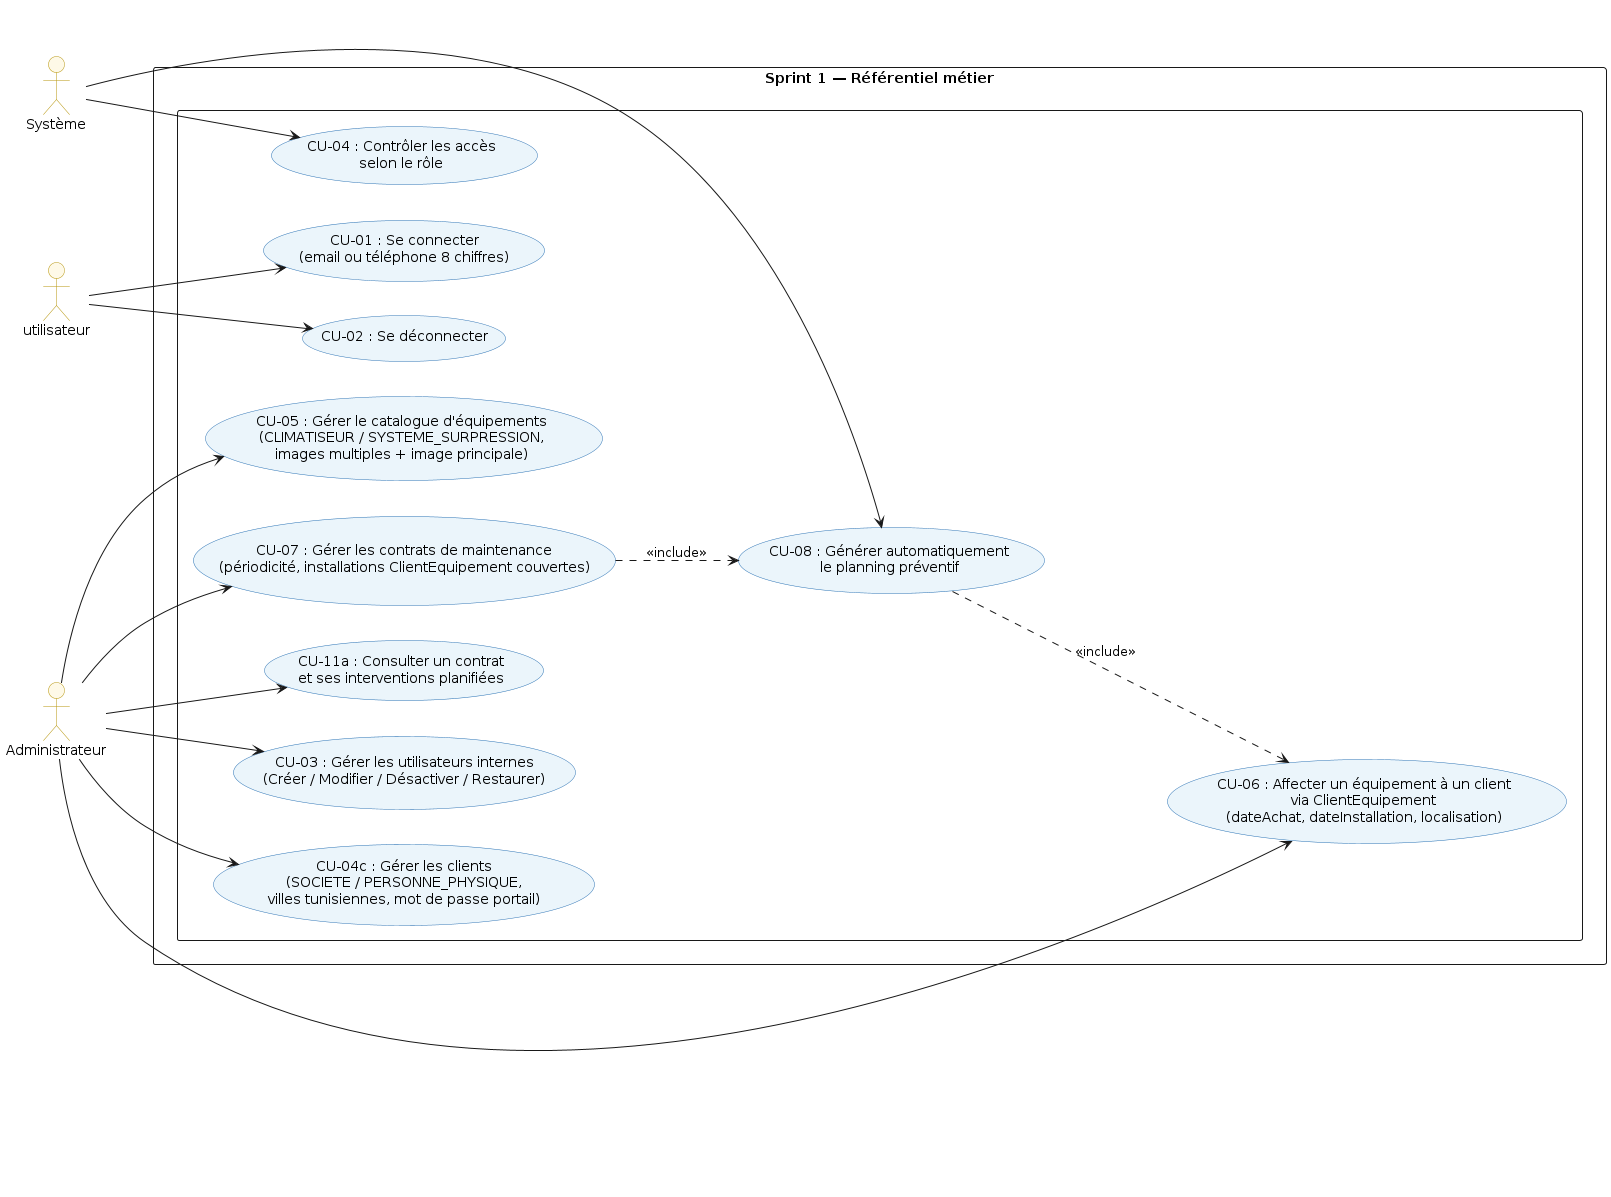
\includegraphics[width=0.70\textwidth]
{Figures/Chapitre3/use_case_sprint1.png}
\caption{Diagramme de cas d'utilisation du Sprint 1}
\label{fig:ch3:usecase_sprint1}
\end{figure}

Acteurs impliqués dans ce sprint :

\textbf{Administrateur} : gestion des utilisateurs, clients, catalogue équipements,
affectation \texttt{ClientEquipement}, contrats.

\textbf{Tout utilisateur} : connexion.

\textit{Comportements automatiques du système :} contrôle d'accès selon le rôle, génération du planning préventif.

\subsection{Description des cas d'utilisation}

\subsubsection{CU-01 : S'authentifier}

\begin{table}[H]
\centering
\caption{CU-01 : S'authentifier}
\label{tab:ch3:cu01}
\begin{tabular}{|p{3.5cm}|p{11cm}|}
\hline
\textbf{Champ} & \textbf{Contenu} \\
\hline
\textbf{Description}
  & Ce cas d'utilisation permet à un utilisateur de s'authentifier dans le système. \\
\hline
\textbf{Acteurs}
  & Administrateur, Technicien, Client \\
\hline
\textbf{Préconditions}
  & L'utilisateur possède un compte valide et actif. \\
\hline
\textbf{Postconditions}
  & L'utilisateur accède à son espace personnel selon son rôle. \\
\hline
\end{tabular}
\end{table}

\textbf{Scénario nominal :}
\begin{enumerate}
    \item L'utilisateur ouvre l'interface de connexion.
    \item Il saisit son identifiant (\textbf{adresse e-mail ou numéro de téléphone à 8 chiffres})
          et son mot de passe.
    \item Le système détecte le type d'identifiant : si l'identifiant contient un « @ »,
          il s'agit d'un e-mail ; sinon, il s'agit d'un numéro de téléphone.
    \item Le système recherche l'utilisateur correspondant dans la base de données.
    \item Le système vérifie le mot de passe.
    \item Le système crée la session et redirige l'utilisateur vers son tableau de bord
          selon son rôle.
\end{enumerate}

\textbf{Scénarios alternatifs :}
\begin{itemize}
    \item Identifiant (e-mail ou téléphone) non reconnu $\rightarrow$ message d'erreur affiché.
    \item Mot de passe incorrect $\rightarrow$ message d'erreur affiché.
    \item Compte inactif (\texttt{actif = false}) $\rightarrow$ accès refusé avec message d'erreur.
\end{itemize}

\subsubsection{CU-03 : Gérer les utilisateurs internes}

\begin{table}[H]
\centering
\caption{CU-03 : Gérer les utilisateurs internes}
\label{tab:ch3:cu03}
\begin{tabular}{|p{3.5cm}|p{11cm}|}
\hline
\textbf{Champ} & \textbf{Contenu} \\
\hline
\textbf{Description}
  & Ce cas d'utilisation permet à l'administrateur de gérer les comptes des utilisateurs
    internes (administrateurs et techniciens). \\
\hline
\textbf{Acteur principal}
  & Administrateur \\
\hline
\textbf{Préconditions}
  & L'administrateur est authentifié. \\
\hline
\textbf{Postconditions}
  & Les modifications sont enregistrées dans la base de données. \\
\hline
\end{tabular}
\end{table}

\textbf{Fonctionnalités :}
\begin{itemize}
    \item Créer un utilisateur interne (prénom, nom, e-mail, téléphone, rôle, mot de passe) ;
    \item Modifier un utilisateur existant ;
    \item Désactiver un utilisateur (soft-delete : \texttt{actif = false}) ;
    \item Restaurer un utilisateur désactivé (\texttt{actif = true}) ;
    \item Consulter la liste des utilisateurs avec filtres.
\end{itemize}

\textbf{Scénario nominal :} Le scénario consiste à saisir les informations requises ou à sélectionner un utilisateur existant, à valider les données côté contrôleur (unicité de l'e-mail, chiffrement du mot de passe), puis à enregistrer la modification en base et à actualiser l'affichage.

\textbf{Règles de gestion :}
\begin{itemize}
    \item Chaque utilisateur interne doit avoir un e-mail unique.
    \item Le mot de passe est chiffré avant stockage.
    \item Un utilisateur désactivé (\texttt{actif = false}) ne peut plus se connecter.
    \item L'action « Restaurer » remet \texttt{actif = true}.
    \item Les comptes clients ne sont pas gérés ici --- ils appartiennent au module Clients.
\end{itemize}

\subsubsection{CU-04 : Gérer les clients}

\begin{table}[H]
\centering
\caption{CU-04 : Gérer les clients}
\label{tab:ch3:cu04}
\begin{tabular}{|p{3.5cm}|p{11cm}|}
\hline
\textbf{Champ} & \textbf{Contenu} \\
\hline
\textbf{Description}
  & Ce cas d'utilisation permet à l'administrateur de gérer les fiches clients. \\
\hline
\textbf{Acteur principal}
  & Administrateur \\
\hline
\textbf{Préconditions}
  & L'administrateur est authentifié. \\
\hline
\textbf{Postconditions}
  & Les modifications sont enregistrées dans la base de données. \\
\hline
\end{tabular}
\end{table}

\textbf{Fonctionnalités :}
\begin{itemize}
    \item Créer un client de type \textbf{société} (champs : raison sociale societe, nom du contact)
          ou \textbf{personne physique} (champs : prenom, nom) ;
    \item Renseigner e-mail, téléphone, adresse, ville (liste tunisienne), mot de passe portail ;
    \item Modifier et supprimer un client ;
    \item Consulter la liste avec filtres.
\end{itemize}

\textbf{Règles de gestion :}
\begin{itemize}
    \item Le type \texttt{SOCIETE} requiert le champ societe (raison sociale).
    \item Le type \texttt{PERSONNE\_PHYSIQUE} requiert les champs prenom et nom.
    \item L'e-mail doit être unique dans le système.
    \item Chaque client dispose d'un mot de passe pour accéder au portail client.
\end{itemize}

\subsubsection{CU-05 : Gérer le catalogue d'équipements}

\begin{table}[H]
\centering
\caption{CU-05 : Gérer le catalogue d'équipements}
\label{tab:ch3:cu05}
\begin{tabular}{|p{3.5cm}|p{11cm}|}
\hline
\textbf{Champ} & \textbf{Contenu} \\
\hline
\textbf{Description}
  & Ce cas d'utilisation permet à l'administrateur de gérer le catalogue global d'équipements,
    indépendant de tout client. \\
\hline
\textbf{Acteur principal}
  & Administrateur \\
\hline
\textbf{Préconditions}
  & L'administrateur est authentifié. \\
\hline
\textbf{Postconditions}
  & L'équipement est enregistré dans le catalogue. \\
\hline
\end{tabular}
\end{table}

\textbf{Fonctionnalités :}
\begin{itemize}
    \item Créer un équipement avec : référence, type (\texttt{CLIMATISEUR} ou
          \texttt{SYSTEME\_SURPRESSION}), marque, modèle, numéro de série, description ;
    \item Ajouter plusieurs images (\texttt{EquipmentImage}) dont une image principale
          (\texttt{isMain = true}) ;
    \item Modifier et supprimer un équipement ;
    \item Consulter le catalogue avec filtres par type et marque.
\end{itemize}

\textbf{Règles de gestion :}
\begin{itemize}
    \item Le catalogue est global : un équipement n'appartient pas à un client spécifique.
    \item Le numéro de série est unique.
    \item Une seule image est désignée comme image principale.
\end{itemize}

\subsubsection{CU-06 : Affecter un équipement à un client (\texttt{ClientEquipement})}

\begin{table}[H]
\centering
\caption{CU-06 : Affecter un équipement à un client}
\label{tab:ch3:cu06}
\begin{tabular}{|p{3.5cm}|p{11cm}|}
\hline
\textbf{Champ} & \textbf{Contenu} \\
\hline
\textbf{Description}
  & Ce cas d'utilisation permet à l'administrateur de créer un enregistrement
    \texttt{ClientEquipement} qui matérialise l'installation d'un équipement du catalogue
    chez un client. \\
\hline
\textbf{Acteur principal}
  & Administrateur \\
\hline
\textbf{Préconditions}
  & L'administrateur est authentifié ; le client existe ; l'équipement existe dans le catalogue. \\
\hline
\textbf{Postconditions}
  & Un enregistrement \texttt{ClientEquipement} est créé en base de données. \\
\hline
\end{tabular}
\end{table}

\textbf{Scénario nominal :} L'administrateur sélectionne l'équipement et le client, renseigne la date d'installation et valide ; le contrôleur vérifie l'existence des deux entités et l'absence de doublon avant d'enregistrer le \texttt{ClientEquipement}.

\textbf{Règles de gestion :}
\begin{itemize}
    \item La date d'installation est obligatoire. La localisation est facultative.
    \item Un même équipement peut être affecté à plusieurs clients différents
          (via des enregistrements \texttt{ClientEquipement} distincts).
    \item L'affectation ne modifie pas le catalogue global.
\end{itemize}

\subsubsection{CU-07 : Gérer les contrats de maintenance}

\begin{table}[H]
\centering
\caption{CU-07 : Gérer les contrats de maintenance}
\label{tab:ch3:cu07}
\begin{tabular}{|p{3.5cm}|p{11cm}|}
\hline
\textbf{Champ} & \textbf{Contenu} \\
\hline
\textbf{Description}
  & Ce cas d'utilisation permet à l'administrateur de créer un contrat de maintenance
    couvrant des installations \texttt{ClientEquipement}. \\
\hline
\textbf{Acteur principal}
  & Administrateur \\
\hline
\textbf{Préconditions}
  & L'administrateur est authentifié ; le client existe ; des enregistrements
    \texttt{ClientEquipement} existent pour ce client. \\
\hline
\textbf{Postconditions}
  & Le contrat est enregistré en base ; les interventions préventives sont générées
    automatiquement par le Système. \\
\hline
\end{tabular}
\end{table}

\textbf{Scénario nominal :} L'administrateur saisit les informations du contrat (client, dates, périodicité, installations \texttt{ClientEquipement} couvertes) ; le contrôleur vérifie la cohérence des dates et l'appartenance des installations au client, enregistre le contrat dans une transaction et déclenche la génération automatique du planning préventif.

\textbf{Scénarios alternatifs :} En cas d'erreur (dates invalides, installations non rattachées au client ou échec base de données), l'opération est interrompue, la transaction est annulée et un message explicite est affiché.

\textbf{Règles de gestion :}
\begin{itemize}
    \item Un contrat couvre des installations \texttt{ClientEquipement}, et non des équipements
          du catalogue directement.
    \item Le statut est calculé dynamiquement : \texttt{ACTIF} si fin > aujourd'hui + 30 jours ;
          \texttt{BIENTOT\_EXPIRE} si fin entre aujourd'hui et aujourd'hui + 30 jours ;
          \texttt{EXPIRE} si fin < aujourd'hui.
    \item La génération du planning est automatique et ne requiert aucune action manuelle
          de l'administrateur.
\end{itemize}

\subsubsection{CU-08 : Générer automatiquement le planning préventif}

\begin{table}[H]
\centering
\caption{CU-08 : Générer automatiquement le planning préventif}
\label{tab:ch3:cu08}
\begin{tabular}{|p{3.5cm}|p{11cm}|}
\hline
\textbf{Champ} & \textbf{Contenu} \\
\hline
\textbf{Description}
  & Ce cas d'utilisation décrit le traitement automatique déclenché par le système lors
    de la sauvegarde d'un contrat. \\
\hline
\textbf{Déclencheur}
  & Comportement automatique du système \\
\hline
\textbf{Préconditions}
  & Un contrat valide vient d'être enregistré avec ses \texttt{clientEquipementIds[]},
    ses dates et sa périodicité. \\
\hline
\textbf{Postconditions}
  & Les interventions préventives sont créées en base de données pour toute la durée
    du contrat. \\
\hline
\end{tabular}
\end{table}

\textbf{Scénario nominal :} Le système calcule les dates d'intervention selon la périodicité et les installations couvertes, puis génère les interventions préventives dans une transaction unique.

\textbf{Règles de gestion :}
\begin{itemize}
    \item La génération est automatique : elle est déclenchée par la sauvegarde du contrat,
          non par une action manuelle.
    \item Une intervention préventive est générée pour chaque couple
          (date, \texttt{ClientEquipement} couvert).
    \item Périodicités : mensuelle (12/an), trimestrielle (4/an), semestrielle (2/an),
          annuelle (1/an).
\end{itemize}

% ─────────────────────────────────────────────────────────────────────────────
\section{Conception}

\subsection{Diagramme de classes du Sprint 1}

\begin{figure}[H]
\centering
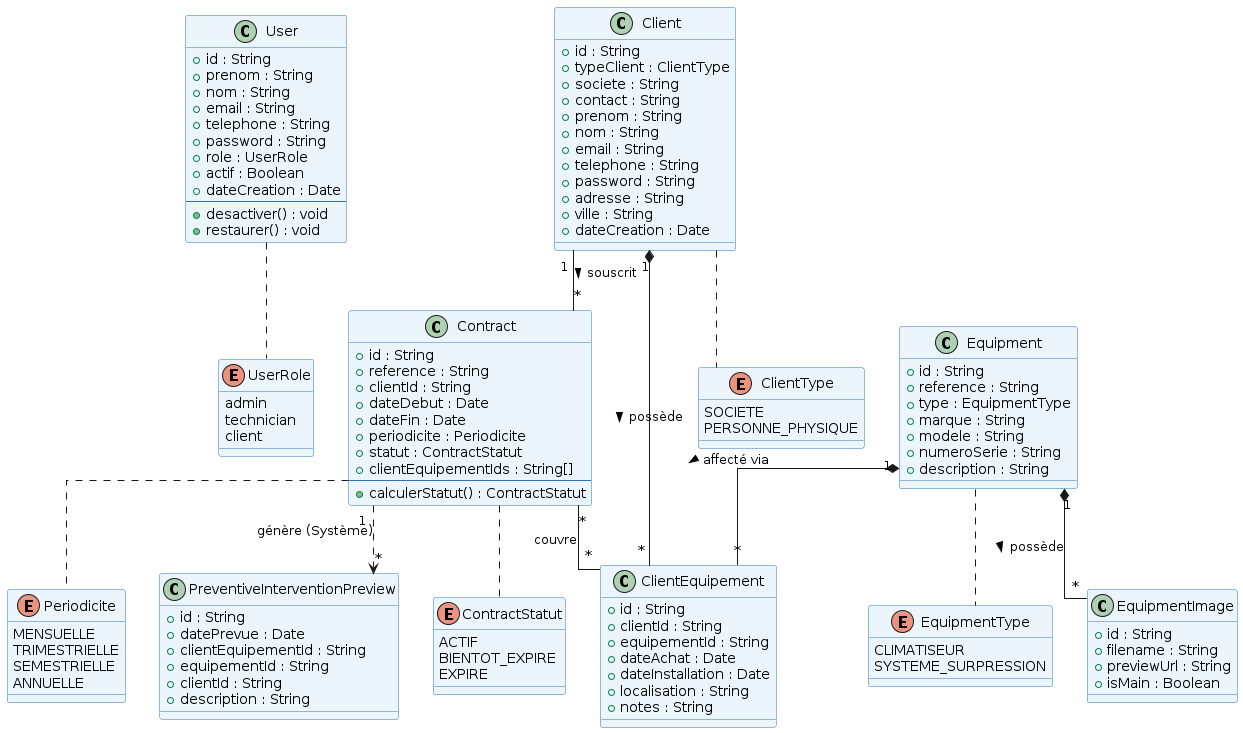
\includegraphics[width=0.70\textwidth]{Figures/Chapitre3/class_diagram_sprint1.png}
\caption{Diagramme de classes du Sprint 1}
\label{fig:ch3:class_sprint1}
\end{figure}

Les entités impliquées dans ce sprint sont : \texttt{User}, \texttt{Client}, \texttt{Equipment},
\texttt{EquipmentImage}, \texttt{ClientEquipement}, \texttt{Contract}, \texttt{Intervention}
(préventive générée automatiquement).

\subsection{Diagrammes de séquence}

\subsubsection{Diagramme de séquence : Connexion (email ou téléphone)}

\begin{figure}[H]
\centering
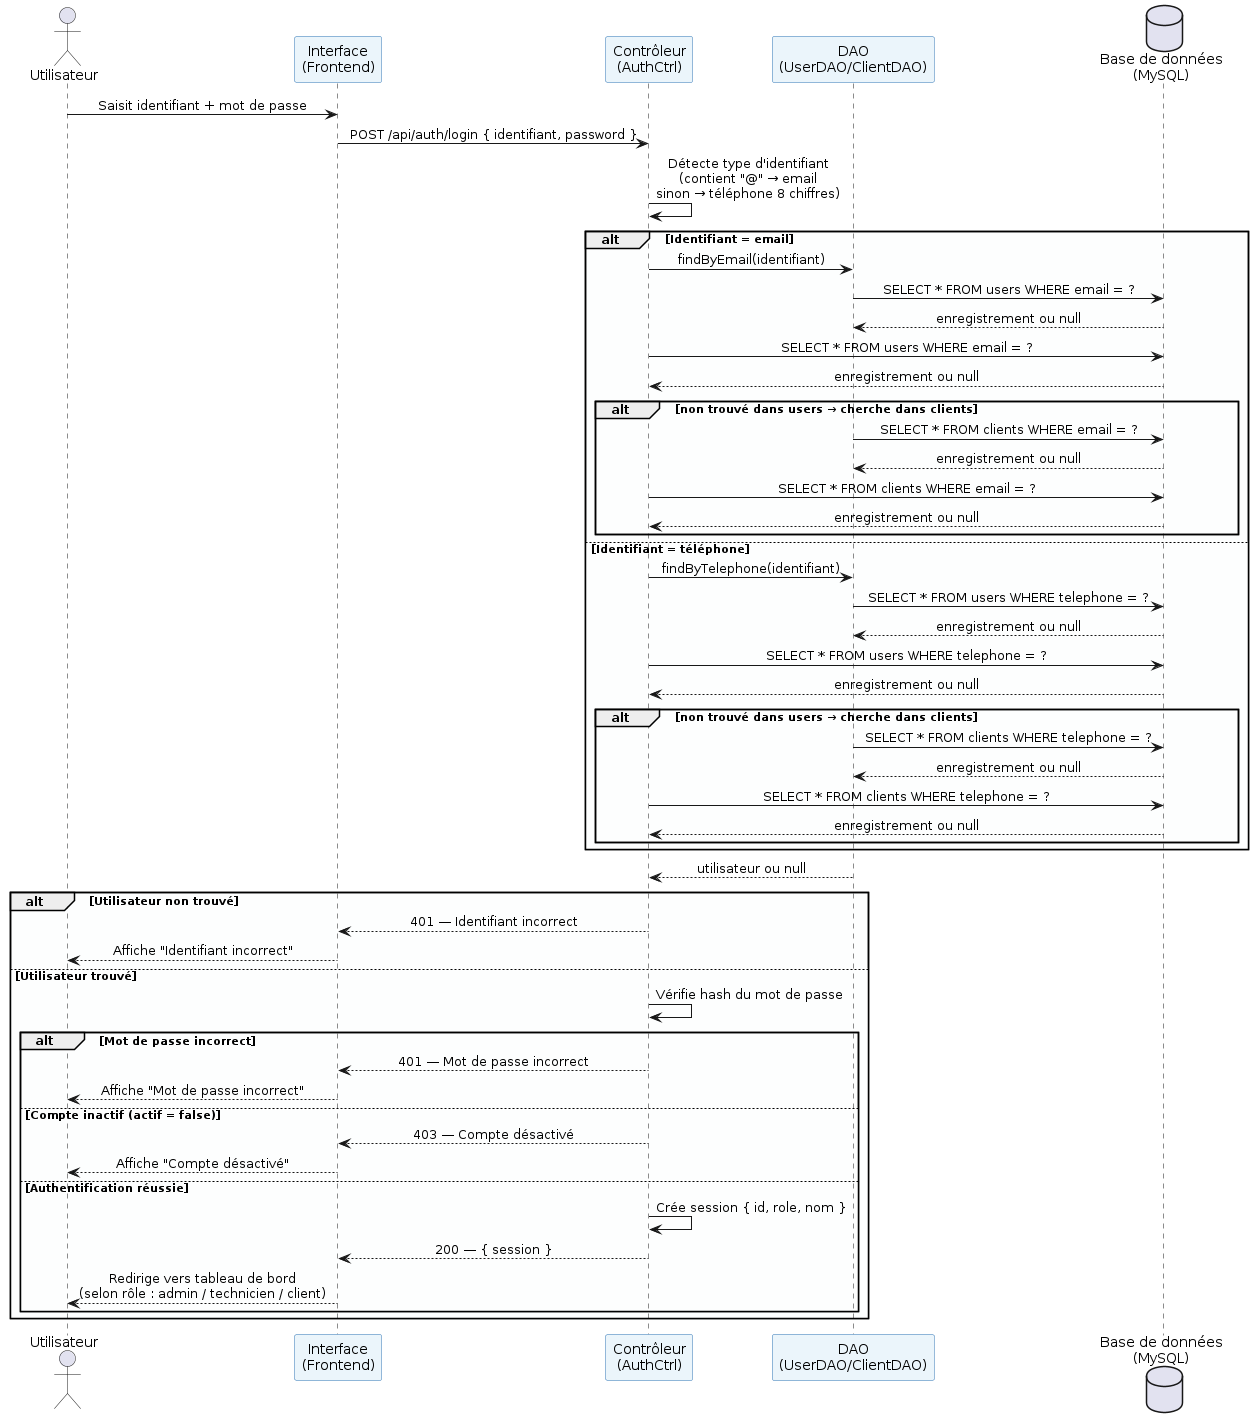
\includegraphics[width=0.70\textwidth]{Figures/Chapitre3/seq_connexion_sprint1.png}
\caption{Diagramme de séquence : Connexion}
\label{fig:ch3:seq_connexion}
\end{figure}

\subsubsection{Diagramme de séquence : Ajout équipement et gestion des images}

\begin{figure}[H]
\centering
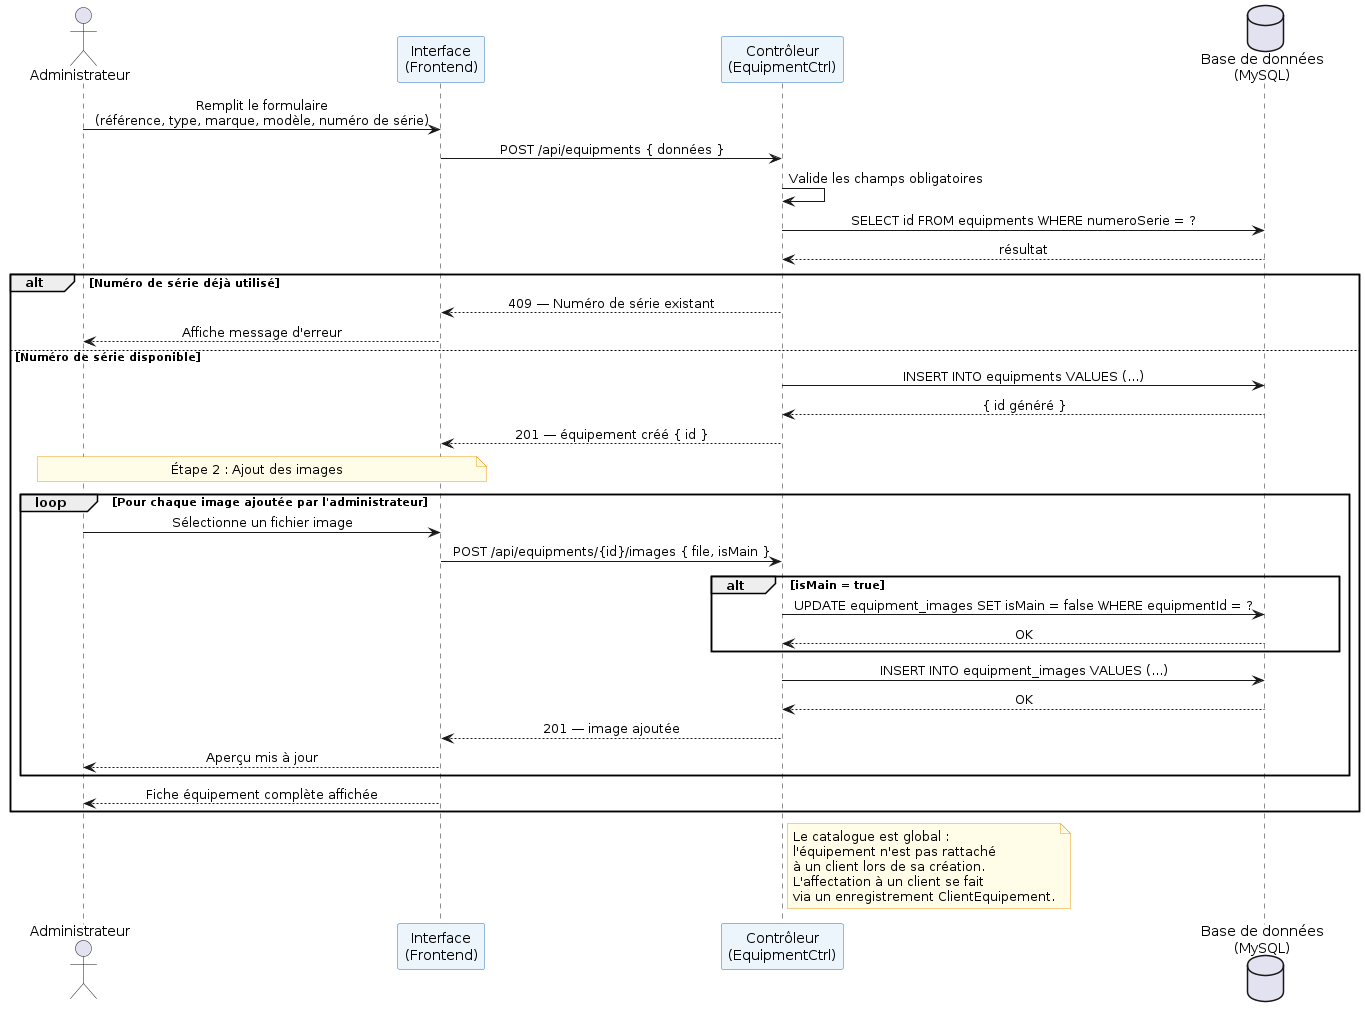
\includegraphics[width=0.70\textwidth]{Figures/Chapitre3/seq_ajoutequip_sprint1.png}
\caption{Diagramme de séquence : Ajout équipement et gestion des images}
\label{fig:ch3:seq_ajout_equipement}
\end{figure}

% ─────────────────────────────────────────────────────────────────────────────
\section{Réalisation}

\begin{figure}[H]
    \centering
    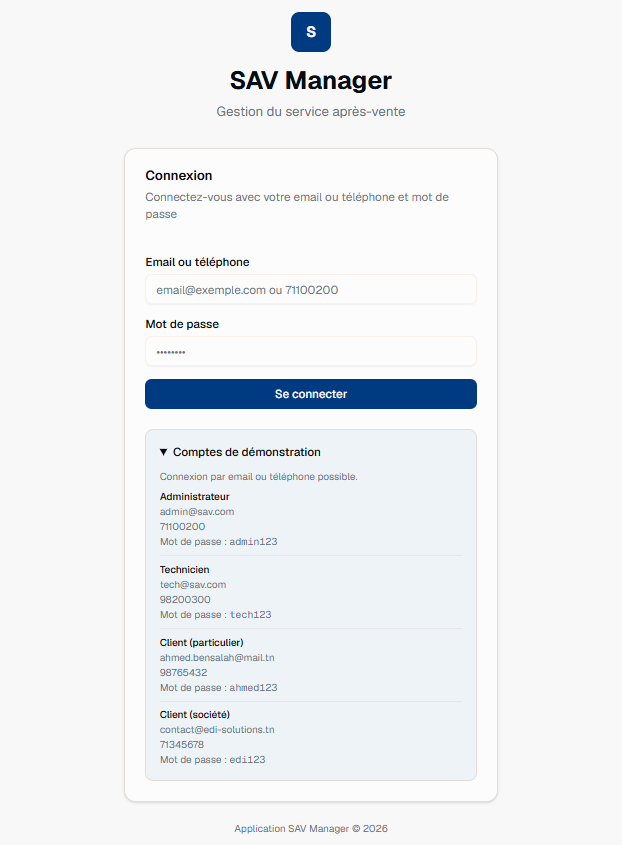
\includegraphics[width=0.74\textwidth]{Figures/Chapitre3/login.png}
    \caption{Capture d'écran : interface de connexion}
    \label{fig:ch3:login}
\end{figure}

\begin{figure}[H]
    \centering
    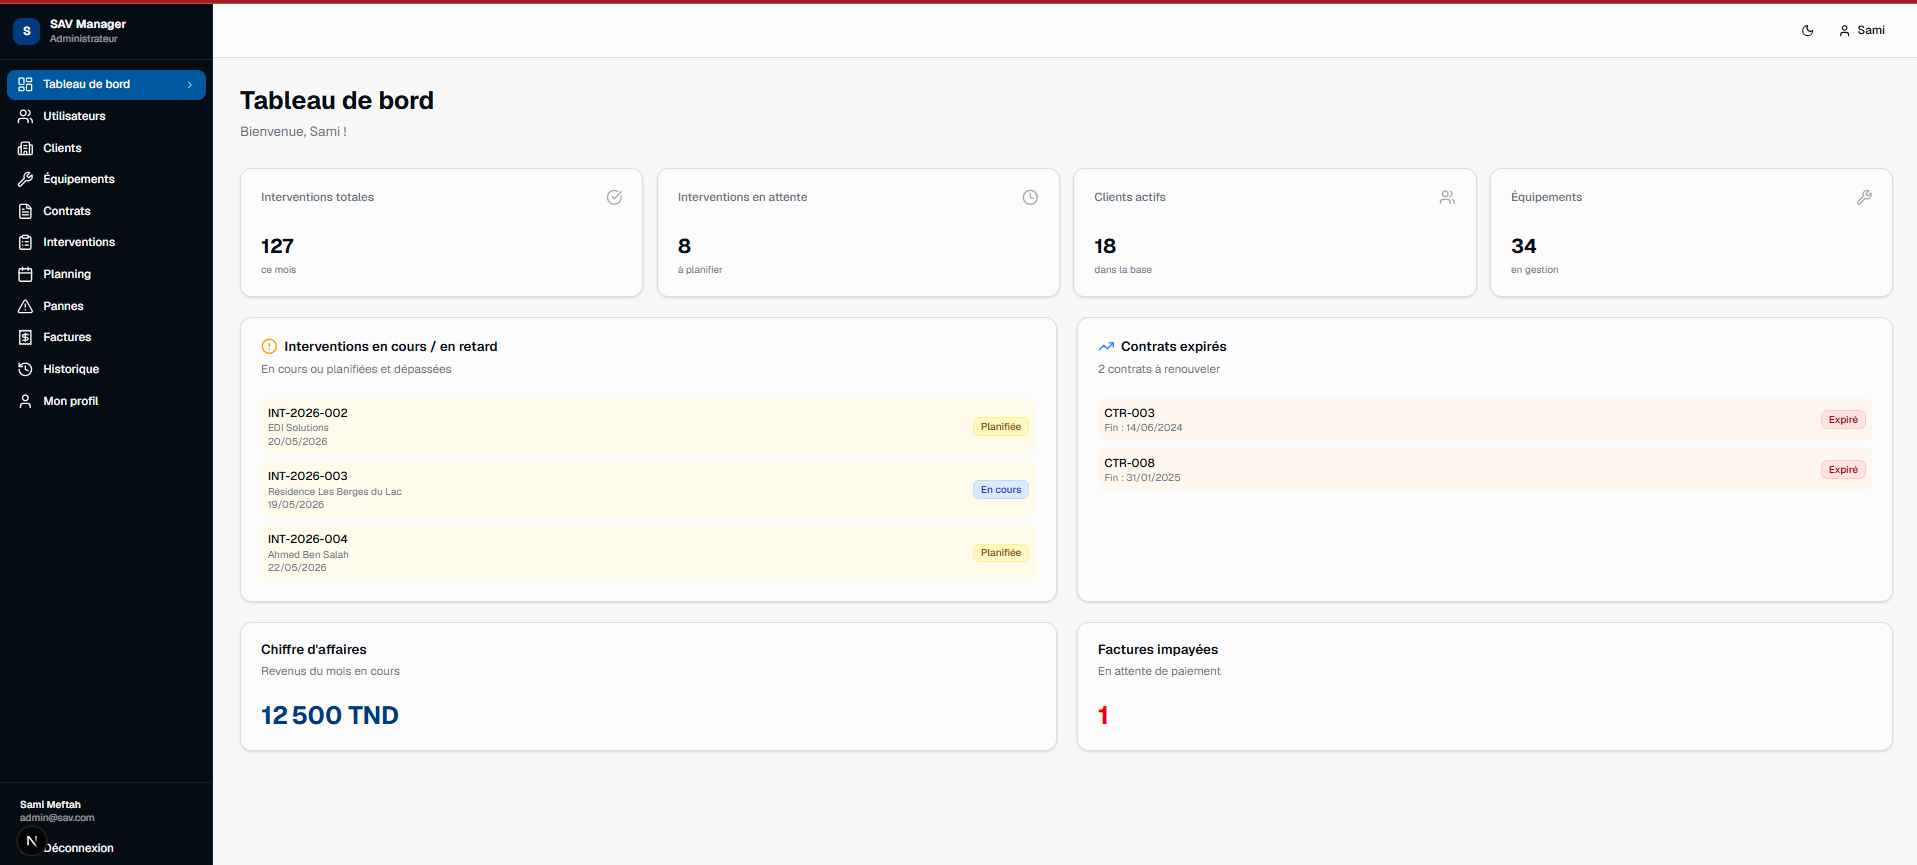
\includegraphics[width=0.74\textwidth]{Figures/Chapitre3/dashboardadmin.png}
    \caption{Capture d'écran : tableau de bord administrateur}
    \label{fig:ch3:dashboard_admin}
\end{figure}

\begin{figure}[H]
    \centering
    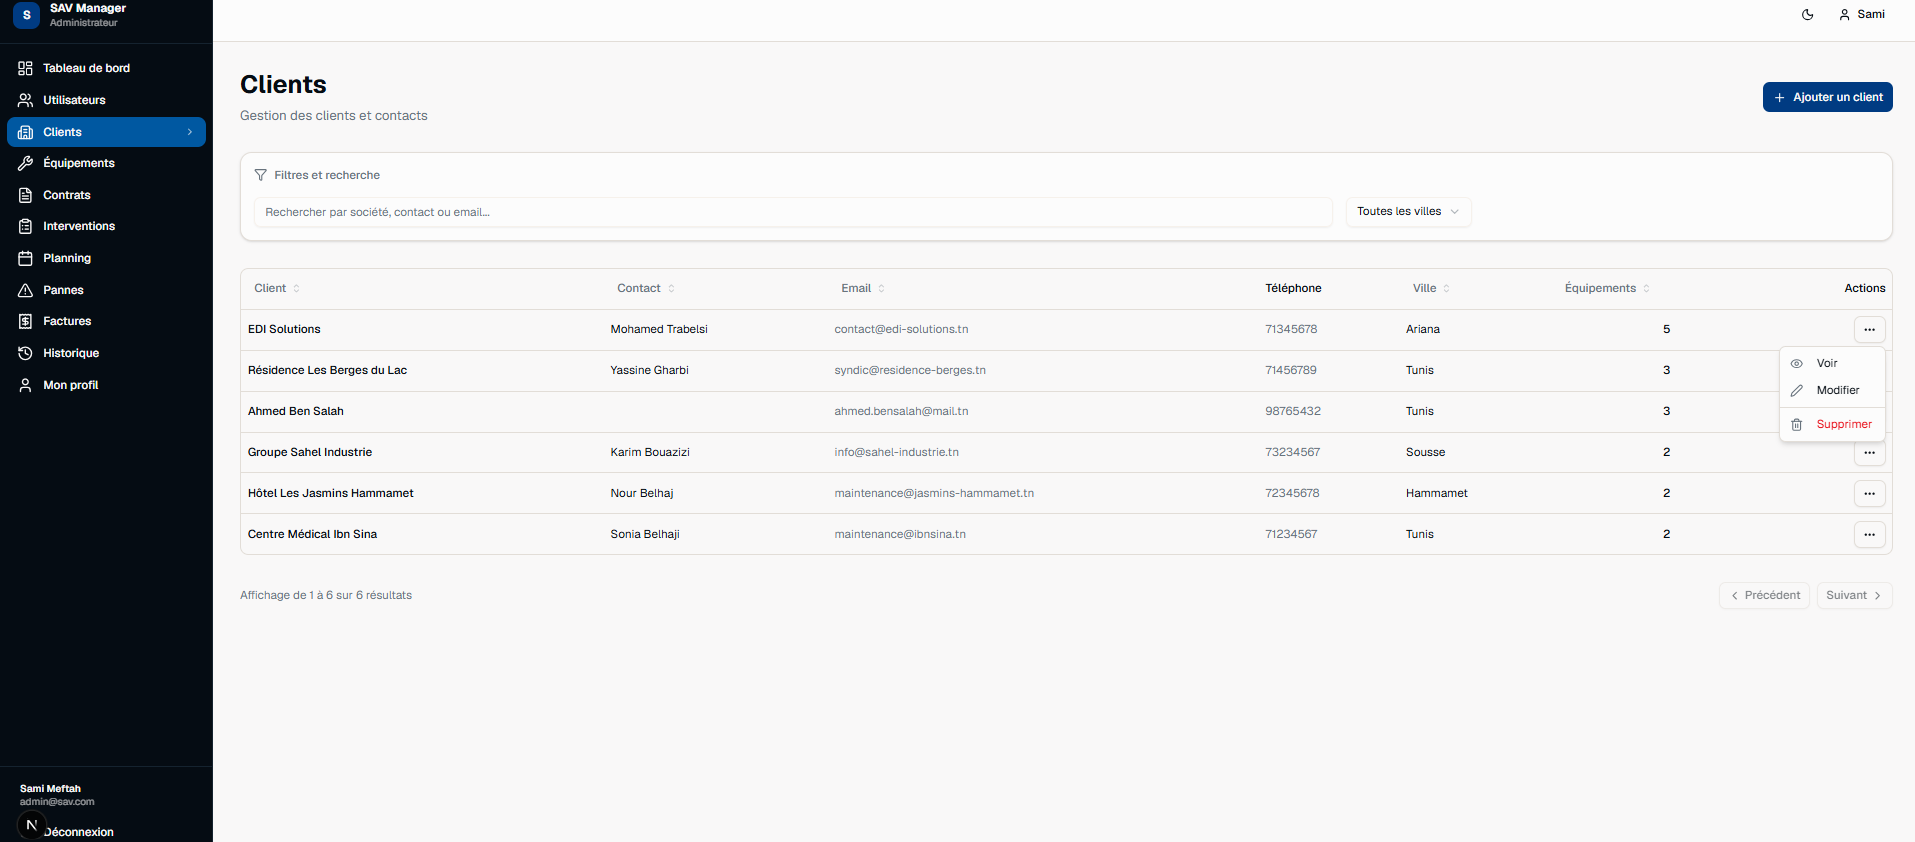
\includegraphics[width=0.74\textwidth]{Figures/Chapitre3/gestclient.png}
    \caption{Capture d'écran : gestion des clients}
    \label{fig:ch3:gestion_clients}
\end{figure}

\begin{figure}[H]
    \centering
    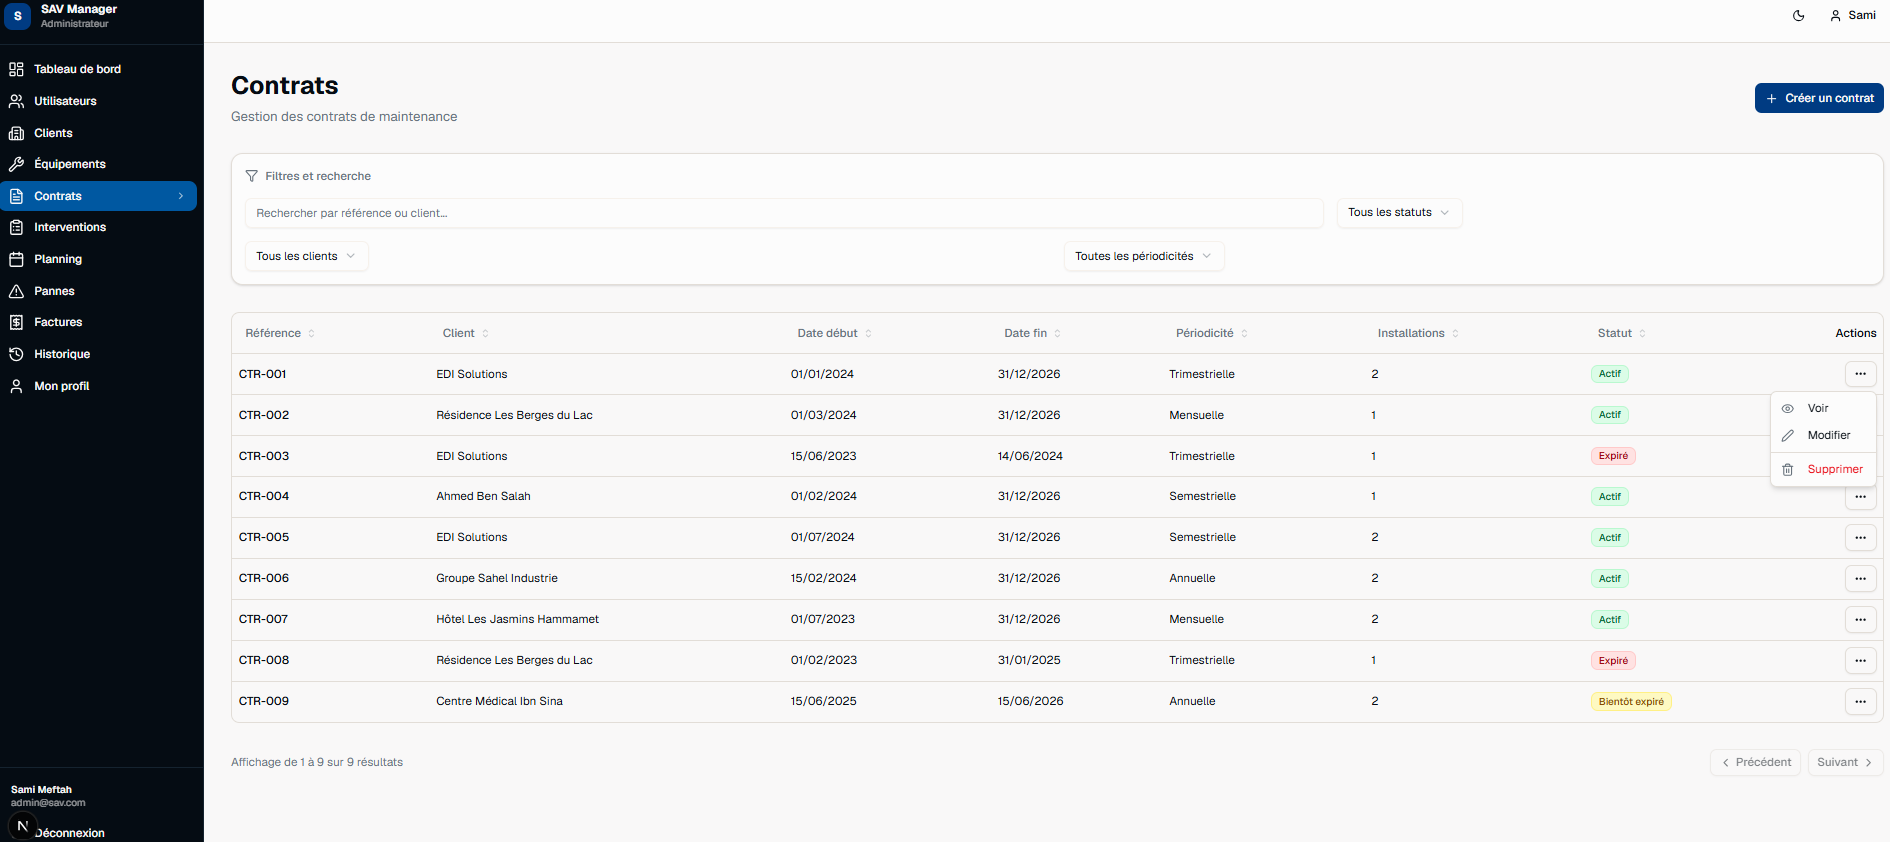
\includegraphics[width=0.74\textwidth]{Figures/Chapitre3/gestcontrat.png}
    \caption{Capture d'écran : gestion des contrats}
    \label{fig:ch3:gestion_contrats}
\end{figure}

% ─────────────────────────────────────────────────────────────────────────────
\section*{Conclusion}

Ce sprint a permis de mettre en place les fondations du système : l'authentification sécurisée
par e-mail ou téléphone, la gestion des référentiels métier (utilisateurs, clients, catalogue
équipements avec images, affectation \texttt{ClientEquipement}), la gestion des contrats et la
génération automatique du planning préventif par le Système. Le chapitre suivant présente le
Sprint 2 dédié à la gestion des interventions et des pannes.
